\documentclass[12pt]{report} % ---- COMPILE WITH XeLaTeX for Unicode!!! ----
\usepackage[a4paper, top=1in, bottom=1in, left=1.5in, right=1in]{geometry} % Set margins
\usepackage{setspace} % allows \doublespacing & \singlespacing
\usepackage{parskip} % enables non-indented paragraphs with a blank line
\UseRawInputEncoding

\usepackage{listings}
\usepackage{xcolor}
% enables graphics, all figures and images should be in the /figures/ folder:
\usepackage{graphicx}

\def\changemargin#1#2{\list{}{\rightmargin#2\leftmargin#1}\item[]}
\let\endchangemargin=\endlist 
% enhanced maths symbols and syntax:
\usepackage{amsmath}
\usepackage{amssymb}
\usepackage{amsthm} % if you need mathematical definitions and theorems

\usepackage[ruled]{algorithm2e} % allow for algorithms in pseudocode
\usepackage{listings} % allow for source code algorithms/listings
\lstset{basicstyle=\footnotesize, frame=single, numbers=left} % customise listing style

% Customise chapter headings so they are of the format: 1. Introduction
\usepackage{titlesec}
\titleformat{\chapter}[block]
  {\normalfont\huge\bfseries}{\thechapter.}{1em}{\Huge}
\titlespacing*{\chapter}{0pt}{-20pt}{20pt}

% Setup bibliography - add file to project named bibliography.bib
% can create this from Zotero, Mendeley, refworks, etc
\usepackage{natbib}
\bibliographystyle{agsm}
\setcitestyle{authoryear,open={(},close={)}, aysep={,}}

\usepackage{hyperref} % add links to document



% Colored Python listing from https://www.overleaf.com/learn/latex/Code_listing
\definecolor{codegreen}{rgb}{0,0.6,0}
\definecolor{codegray}{rgb}{0.5,0.5,0.5}
\definecolor{codepurple}{rgb}{0.58,0,0.82}
\definecolor{backcolour}{rgb}{0.95,0.95,0.92}
 
\lstdefinestyle{mystyle}{
    backgroundcolor=\color{backcolour},   
    commentstyle=\color{codegreen},
    keywordstyle=\color{magenta},
    numberstyle=\tiny\color{codegray},
    stringstyle=\color{codepurple},
    basicstyle=\ttfamily\footnotesize,
    breakatwhitespace=false,         
    breaklines=true,                 
    captionpos=b,                    
    keepspaces=true,                 
    numbers=left,                    
    numbersep=5pt,                  
    showspaces=false,                
    showstringspaces=false,
    showtabs=false,                  
    tabsize=2
}
\lstset{style=mystyle}



\doublespacing
\begin{document}

% 

\begin{titlepage}
	\topskip0pt
	\vspace*{\fill}

	\begin{center}

		
\includegraphics[width=0.6\textwidth]{images/logo.png}

		\Huge
		\textbf{Evolutionary Algorithms}
		\vspace{0.5cm}

		\Large

		\textbf{ \href{mailto:mq06861@st.habib.edu.pk}{Muhammad Meesum Ali Qazalbash - mq06861}}\\
		\textbf{ \href{mailto:@st.habib.edu.pk}{{Ibrahim - ms06948}}}

		\today
		\vspace{0.5cm}

		CS451 - Computational Intelligence

		\vspace{0.5cm}
		\large
		Assignment 1
	\end{center}

	\vspace*{\fill}
\end{titlepage}

% 


\pagenumbering{roman} % Roman numeral page numbering up to the first page of introduction
\setcounter{page}{2} % Start at "ii", to count title page as "i"

\chapter{Abstract} % \chapter* means the chapter is not in the contents or numbered
The purpose of this assignment is to gather an insight of stochastic optimization using Evolutionary Algorithms (EA). This exercise will enable us to address some known computing problems that map to several real-world problems and are known to be computationally hard.
\tableofcontents

\chapter{Code}
Complete code can be found at:\\
\url{https://github.com/hs05888/CS451-Evolutionary-Algorithms}
\section{Genetic Algorithm}
\pagenumbering{arabic} % Introduction starts at page 1.

\begin{changemargin}{-3cm}{-2cm}

	% \lstinputlisting{../Code/Evolution/evolution.py}

	\begin{lstlisting}[language=python, caption= {Initializing the evolution class with attributes}, captionpos=b]
class Evolution:
    def __init__(
            self,
            problem: Problem,  # The problem to be solved
            selectionMethod1: int = 0,  # parent selection method?
            selectionMethod2: int = 0,  # survivor selection method?
            population_size: int = 30,  # How many chromosomes?
            number_of_offsprings: int = 10,  # How many offspring?
            number_of_generations: int = 100,  # How many generations?
            mutation_rate: float = 0.50,  # Mutation rate
    ):
    
        self.population_size = population_size # Number of chromosomes
        self.number_of_generations = number_of_generations

        self.number_of_offsprings = number_of_offsprings # Number of offsprings per gen
        self.mutation_rate = mutation_rate  # Probability of mutation

        # Selection methods for the parents and survivors
        self.selectionMethod1 = selectionMethod1
        self.selectionMethod2 = selectionMethod2
        
        # Selection schemes
        self.selectionSchemes = SelectionSchemes(
            population_size=population_size,
            fitness_function=problem.fitness_function)
            
        self.chromosome = problem.chromosome  # Some random chromosome
        self.fitness_function = problem.fitness_function  # Fitness function
        
        self.mutate = problem.mutate  # Mutation function for the chromosome
        self.crossover = problem.crossover  # Crossover function for two chromosomes
};
\end{lstlisting}
\end{changemargin}

\vspace{1cm}

\begin{changemargin}{-3cm}{-2cm}

	\begin{lstlisting}[language=python, caption= {Initial population}, captionpos=b]
    # Initial population of chromosomes
    def initial_population(self):
        return [self.chromosome() for _ in range(self.population_size)]
\end{lstlisting}
\end{changemargin}


\vspace{1cm}

\begin{changemargin}{-3cm}{-2cm}

	\begin{lstlisting}[language=python, caption= {Fittest chromosome}, captionpos=b]
    # Get the fittest chromosome
    def getBestIndividual(self, population):
        return max(population, key=self.fitness_function)
\end{lstlisting}
\end{changemargin}


\vspace{1cm}

\begin{changemargin}{-3cm}{-2cm}

	\begin{lstlisting}[language=python, caption= {Best fitness}, captionpos=b]
    # Get the best fitness of the population
    def getBestFitness(self, population):
        best_chromosone = self.getBestIndividual(population)
        return self.fitness_function(best_chromosone)
\end{lstlisting}
\end{changemargin}


\newpage

\begin{changemargin}{-3cm}{-2cm}

	\begin{lstlisting}[language=python, caption= { Every offspring has a chance of being mutated}, captionpos=b]
    def get_offspring(self, parent, parent2): # Get the offspring of two parents
        child = self.crossover(parent, parent2)
        if (random.random() < self.mutation_rate):
            child = self.mutate(child)
        return child
\end{lstlisting}
\end{changemargin}

\vspace{1cm}

\begin{changemargin}{-3cm}{-2cm}

	\begin{lstlisting}[language=python, caption= {Select two parents and add their offspring to the population}, captionpos=b]
    def breed_parents(self, population: list): # Breed the parents
        for _ in range(self.number_of_offsprings):
            parents = random.sample(population, 2)
            child = self.get_offspring(parents[0], parents[1])
            population.append(child)
        return population
\end{lstlisting}
\end{changemargin}

\vspace{1cm}

\begin{changemargin}{-3cm}{-2cm}

	\begin{lstlisting}[language=python, caption= {First we select parents using the selection method. Then we breed the parents to get the offsprings. The length of population will increase because of this. Then we select survivors using the selection method. The length of population will now equal population size}]
    # Get the next generation using selection methods and breeding
    def next_generation(self, population):
        selection_methods = [
            self.fitness_proportionate, self.ranked_selection,
            self.tournament_selection, self.truncation, self.random_selection
        ]

        parents = selection_methods[self.selectionMethod1](population)
        new_population = self.breed_parents(parents)
        survivors = selection_methods[self.selectionMethod2](new_population)
        return survivors
\end{lstlisting}
\end{changemargin}


\vspace{1cm}

\begin{changemargin}{-3cm}{-2cm}

	\begin{lstlisting}[language=python, caption= {Run the evolution}, captionpos=b]

    # Get population of generation
    def step(self, population):
        '''
        Get the best fitness of the population
        Then we get the next generation using selection methods and breeding
        '''
        best_fitness = self.getBestFitness(population)
        population = self.next_generation(population)
        return population, best_fitness

    # Run the evolution
    def run(self):

        population = self.initial_population()
        fitness_lst = []
        for _ in range(self.number_of_generations):
            population, best_fitness = self.step(population)
            fitness_lst.append(best_fitness)

        return fitness_lst


\end{lstlisting}
\end{changemargin}

\newpage

\subsection{Selection Schemes}



\begin{changemargin}{-3cm}{-2cm}

	\begin{lstlisting}[language=python, caption= {First the population will be sorted according to the fitness of each chromosome. Then the population will be truncated according to the truncation value. The truncation value is a value between 0 and 1. T equals 0.4 means that we will consider 60 percent of the fittest population and select random chromosomes from that 60 percent and make a new population.}, captionpos=b]
    # Truncation selection
    def truncation(self, population, T=0.4):
        N = len(population)
        sorted_population = sorted(population, key=self.fitness_function)
        new_population = []
        for _ in range(self.population_size):
            r = random.randint(int((1 - T) * N), N - 1)
            new_population.append(sorted_population[r])
        return new_population
\end{lstlisting}
\end{changemargin}


\vspace{1cm}

\begin{changemargin}{-3cm}{-2cm}

	\begin{lstlisting}[language=python, caption= {Each chromosome will be assigned a probability of being selected. Such that the probability of a chromosome being selected is (fitness of chromosone) divided by (sum of all fitnesses).}, captionpos=b]
    # Fitness Propotionate Selection
    def fitness_proportionate(self, population):
        fitness_lst = [
            self.fitness_function(chromosone) for chromosone in population
        ]
        total_fitness = sum(fitness_lst)
        probabilities = [fitness / total_fitness for fitness in fitness_lst]
        return random.choices(population,
                              probabilities,
                              k=self.population_size)
\end{lstlisting}
\end{changemargin}



\vspace{1cm}

\begin{changemargin}{-3cm}{-2cm}

	\begin{lstlisting}[language=python, caption= {We will select two random chromosomes from the population and select the chromosome with the highest fitness and  add that chromosone to the new population.}, captionpos=b]
    # Binary Tournament selection
    def tournament_selection(self, population):
        new_population = []
        for _ in range(self.population_size):
            tournament = random.sample(population, 2)
            winner = max(tournament, key=self.fitness_function)
            new_population.append(winner)
        return new_population
\end{lstlisting}
\end{changemargin}



\vspace{1cm}

\begin{changemargin}{-3cm}{-2cm}

	\begin{lstlisting}[language=python, caption= {        The population will be sorted according to the fitness of each chromosome. The probability of a chromosome being selected is  (rank of chromosome) divided by (total number of chromosomes). The fittest invidual will have the highest rank which will be N. The least fit will have the lowest rank which will be 1.}, captionpos=b]
    # Ranked based selection
    def ranked_selection(self, population):
        N = len(population)
        sorted_population = sorted(population, key=self.fitness_function)
        probabilities = [(i + 1) / N for i, _ in enumerate(sorted_population)]
        return random.choices(sorted_population,
                              probabilities,
                              k=self.population_size)
\end{lstlisting}
\end{changemargin}


\vspace{1cm}

\begin{changemargin}{-3cm}{-2cm}

	\begin{lstlisting}[language=python, caption= {Random selection}, captionpos=b]
    def random_selection(self, population):
        return random.choices(population, k=self.population_size)

\end{lstlisting}
\end{changemargin}

\newpage

\section{Travelling Salesman Problem}

\begin{changemargin}{-3cm}{-2cm}

	\begin{lstlisting}[language=python, caption= {Storing the dataset in a adjacency matrix}, captionpos=b]
import tsplib95  # pip install tsplib95

# Change this to your dataset
file = 'Datasets/qa194.tsp'

with open(file) as f:
    text = f.read()  # Read the file

# Parse the file
problem = tsplib95.parse(text)

# Get the graph
graph = (problem.get_graph())

# Get the number of nodes
num_nodes = int(problem.dimension)

matrix = []  # The adjacency matrix

# For each node Get the connections
for node in range(1, num_nodes + 1):
    connections = list(graph[node].keys())
    weights = []
    # For each connection Get the weight
    for city in connections:
        weights.append(graph[node][city]['weight'])
    matrix.append(weights)  # Add the weights to the matrix
\end{lstlisting}
\end{changemargin}


\newpage

\begin{changemargin}{-3cm}{-2cm}

	\begin{lstlisting}[language=python, caption= {TSP class}, captionpos=b]
class TSP(Problem):

    inverse_fitness = True
    # returns a random route of cities
    def chromosome():
        '''The chromosome representation is just a list of cities (a route) '''
        return random.sample(list(range(num_cities)), num_cities)

    # calculates the distance covered in the route
    def fitness_function(route):
        N = len(graph) - 1
        distances = [graph[route[i]][route[i + 1]] for i in range(N)]
        return 1 / sum(distances)

    # mutates the route by swapping two cities
    def mutate(individual):
        indexes = random.sample(list(range(len(individual))), 2)
        swap1, swap2 = indexes[0], indexes[1]
        individual[swap1], individual[swap2] = individual[swap2], individual[
            swap1]
        return individual

    # returns a offspring after breeding two parents
    def crossover(parent1, parent2):
        geneA = int(random.random() * len(parent1))
        geneB = int(random.random() * len(parent1))

        startGene = min(geneA, geneB)
        endGene = max(geneA, geneB)
        childP1 = parent1[startGene:endGene]
        childP2 = [item for item in parent2 if item not in childP1]
        child = childP1 + childP2
        return child


\end{lstlisting}
\end{changemargin}


\section{Knapsack Problem}

\begin{changemargin}{-3cm}{-2cm}

	\begin{lstlisting}[language=python, caption= {Storing the dataset in a list}, captionpos=b]
# Change this to your dataset
file = 'Datasets/f2_l-d_kp_20_878'

# Open the file
openedFile = open(file, "r")
lines = openedFile.read().split('\n')

# Read the first line
number_of_items = int(lines[0].split(' ')[0])
knapsack_capacity = int(lines[0].split(' ')[1])

# Delete the first line
del lines[0]

profits = []
weights = []

# Read the rest of the lines
for i in range(number_of_items):
    line = lines[i].split(' ')
    profits.append(int(line[0]))
    weights.append(int(line[1]))
\end{lstlisting}
\end{changemargin}


\newpage

\begin{changemargin}{-3cm}{-2cm}

	\begin{lstlisting}[language=python, caption= {Knapsack class}, captionpos=b]
class Knapsack(Problem):
    inverse_fitness = False
    def chromosome():  # Returns a list of randomized binary numbers such that 1 in the ith position means that the ith product is selected
        return random.choices([0, 1], k=number_of_items)

    def fitness_function(solution): # Calculates fitness of a solution
        ''' If the solution has a 1 in the ith position, we add the profit of the ith item to the total profit. Fitness is 0, if we exceeed the capacity of the knapsack'''
        total_profit = 0
        total_weight = 0
        for binary, profit, weight in zip(solution, profits, weights):
            if binary == 1:
                total_profit += profit
                total_weight += weight
        
        if total_weight > threshold: return 0
        return total_profit
    # We flip a binary number at random
    def mutate(individual):
        index = random.randint(0, len(individual) - 1)
        individual[index] = int(not individual[index])
        return individual

    def crossover(parent1, parent2):
        geneA = int(random.random() * len(parent1))
        geneB = int(random.random() * len(parent1))
        startGene = min(geneA, geneB)
        endGene = max(geneA, geneB)
        childP1 = parent1[startGene:endGene]
        childP2 = [item for item in parent2 if item not in childP1]
        child = childP1 + childP2
        return child

\end{lstlisting}
\end{changemargin}




\section{Graph Coloring Problem}

\begin{changemargin}{-3cm}{-2cm}

	\begin{lstlisting}[language=python, caption= {Storing the dataset in a adjacency matrix graph}, captionpos=b]
# Change this to your dataset
file = 'Datasets/gcol1.txt'

# Open the file
openedFile = open(file, "r")
lines = openedFile.read().split('\n')

# Reading the first line
num_nodes = int(lines[0].split(' ')[2])
num_edges = int(lines[0].split(' ')[3])

# Deleting the first line
del lines[0]

# Filling the matrix
matrix = [[0] * num_nodes for _ in range(num_nodes)]
# Adding the edges
for i in range(num_edges):
    _, u, v = lines[i].split(' ')
    u = int(u) - 1
    v = int(v) - 1
    matrix[u][v] = 1
    matrix[v][u] = 1
# if same color assigned and vertexes are adjacent return False
def is_valid(individual): 
    for i in range(num_nodes):
        for j in range(i, num_nodes):
            if matrix[i][j] == 1 and individual[i] == individual[j]:
                return False
    return True
\end{lstlisting}
\end{changemargin}


\newpage

\begin{changemargin}{-3cm}{-2cm}

	\begin{lstlisting}[language=python, caption= {Graph Coloring class}, captionpos=b]
class Graph_Coloring(Problem):

    inverse_fitness = True

    def chromosome():
        '''
        A random solution would be 
        assign a different color to each vertex
        '''
        return random.sample(range(num_nodes), num_nodes)

    def fitness_function(individual):
        '''
        If the solution is valid, return the number of colors used.
        If the solution is not valid, fitness is zero
        '''
        if is_valid(individual): return 1 / len(set(individual))
        else: return 0

    def crossover(parent1, parent2):
        position = random.randint(0, num_nodes - 1)
        child = parent1[:position] + parent2[position:]
        return child

    def mutate(individual: list):
        position = random.randint(0, num_nodes - 1)
        individual[position] = random.randint(0, num_nodes - 1)
        return individual

\end{lstlisting}
\end{changemargin}

\newpage

\section{Optimization Class}

\begin{changemargin}{-3cm}{-2cm}

	\begin{lstlisting}[language=python, caption= {Optimization class}, captionpos=b]
class Optimization:

    def __init__(  # Giving some default paramater values
        self,
        problem: Problem,  # The problem to be solved
        population_size: int = 30,  # How many chromosomes?
        number_of_offsprings: int = 10,  # How many offspring?
        number_of_generations: int = 100,  # How many generations?
        mutation_rate: float = 0.50,  # Mutation rate
        number_of_iterations: int = 10,  # How many iterations?
        selection_case: tuple = (0, 0)  # Selection Schemes
    ):
        self.population_size = population_size
        self.number_of_generations = number_of_generations
        self.number_of_iterations = number_of_iterations

        self.number_of_offsprings = number_of_offsprings
        self.problem = problem
        self.mutation_rate = mutation_rate
        self.selection_case = selection_case

    def evolve(self):
        return Evolution(
            population_size=self.population_size,  # number of chromosomes
            number_of_generations=self.number_of_generations,
            number_of_offsprings=self.number_of_offsprings,
            mutation_rate=self.mutation_rate,  # mutation rate
            problem=self.problem,  # problem to be solved
            selectionMethod1=self.selection_case[0],  # parent select method
            selectionMethod2=self.selection_case[1],  # survivor select method
        )
\end{lstlisting}
\end{changemargin}

\newpage

\chapter{Analysis}

\section{Selection Combination Cases}
We have essentially tested out 10 possible cases of different parent and survivor selection methods for the analysis of our evolutionary algorithm and the optimization of some problem
\begin{itemize}
	\item[Case 0. ] FPS and Random
	\item[Case 1. ] Binary Tournament and Truncation
	\item[Case 2. ] Truncation and Truncation
	\item[Case 3. ] Random and Random
	\item[Case 4. ] FPS and Truncation
	\item[Case 5. ] RBS and Binary Tournament
	\item[Case 6. ] Random and Truncation
	\item[Case 7. ] Binary Tournament and FPS
	\item[Case 8. ] Binary Tournament and RBS
	\item[Case 9. ] Truncation and FPS
\end{itemize}

\newpage

\section{Travelling Salesman Problem}

\subsection{Best and Average Fitness So Far}


\begin{itemize}

	\item Case 0:\\
	      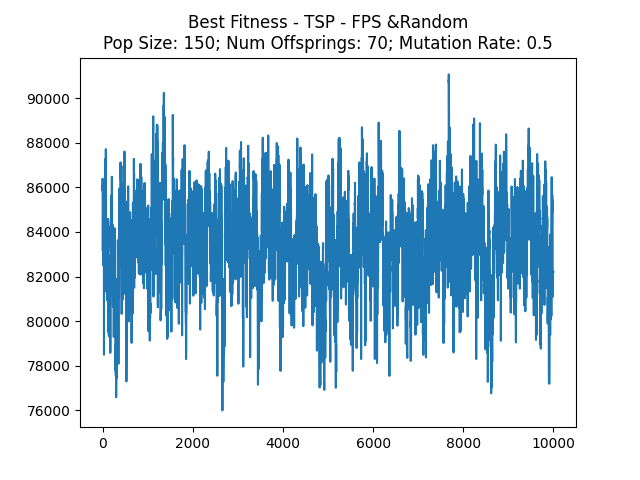
\includegraphics[scale=0.5]{../Analysis/BSF_TSP_0_4_150_70.png}
	      \includegraphics[scale=0.5]{../Analysis/ASF_TSP_0_4_130_70.png}
	      \\Initial fitness:  85734.0
	      \\Final fitness:  84053.0
	      \\Best Average Fitness: 81636.8
	      \\We see that there are many random spikes, the plot doesnt seem to converge at any one value.
	\item Case 1:\\
	      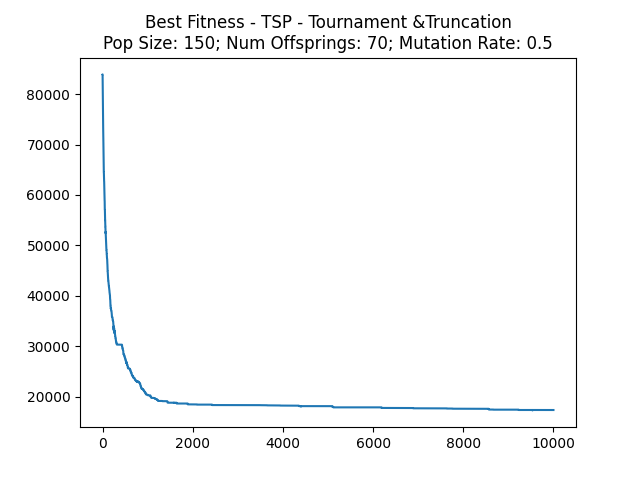
\includegraphics[scale=0.5]{../Analysis/BSF_TSP_2_3_150_70.png}
	      %   \includegraphics[scale=0.5]{../Analysis/ASF_TSP_2_3_150_70.png}
	      \\Initial fitness:  85380.0
	      \\Final fitness:  14510.999999999998
	      \\Best Average Fitness: 15372.6
	      \\The value seems to converge, then have a steady value a bit after 2000 generation.
	\item Case 2:\\
	      %   \includegraphics[scale=0.5]{../Analysis/BSF_TSP_3_3_100_70.png}
	      %   \includegraphics[scale=0.5]{../Analysis/ASF_TSP_3_3_120_70.png}
	      \\Initial fitness:  86046.0
	      \\Final fitness:  14817.999999999998
	      \\Best Average Fitness: 17596.6
	      \\The value seems to converge, then have a steady value after 2000 generation.
	\item Case 3:\\
	      %   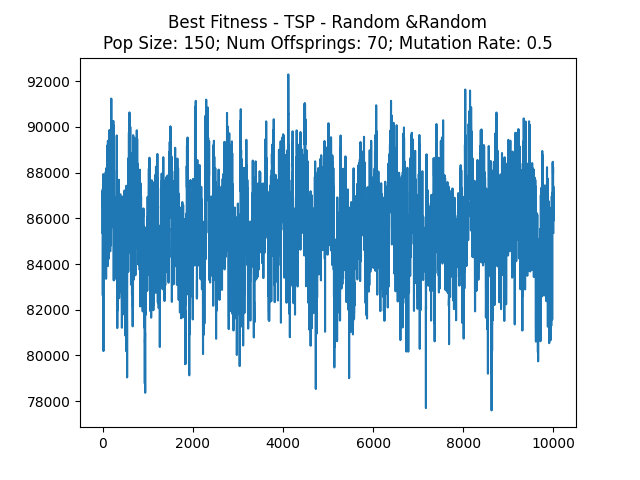
\includegraphics[scale=0.5]{../Analysis/BSF_TSP_4_4_150_70.png}
	      \includegraphics[scale=0.5]{../Analysis/ASF_TSP_4_4_150_70.png}
	      \\Initial fitness:  84833.0
	      \\Final fitness:  84483.0
	      \\Best Average Fitness: 83700.7
	      \\We see that there are many random spikes, the plot doesnt seem to converge at any one value.
	\item Case 4:\\
	      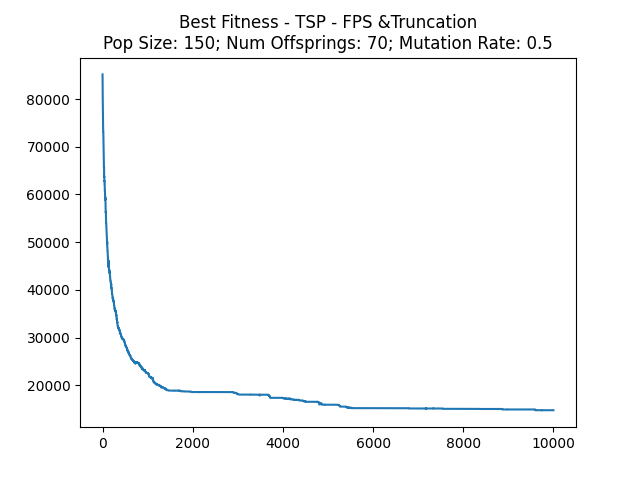
\includegraphics[scale=0.5]{../Analysis/BSF_TSP_0_3_150_70.png}
	      \includegraphics[scale=0.5]{../Analysis/ASF_TSP_0_3_150_70.png}
	      \\Initial fitness:  80943.0
	      \\Final fitness:  17170.0
	      \\Best Average Fitness: 16992.6
	      \\The value seems to converge, then have a steady value after 2000 generation.
	\item Case 5:\\
	      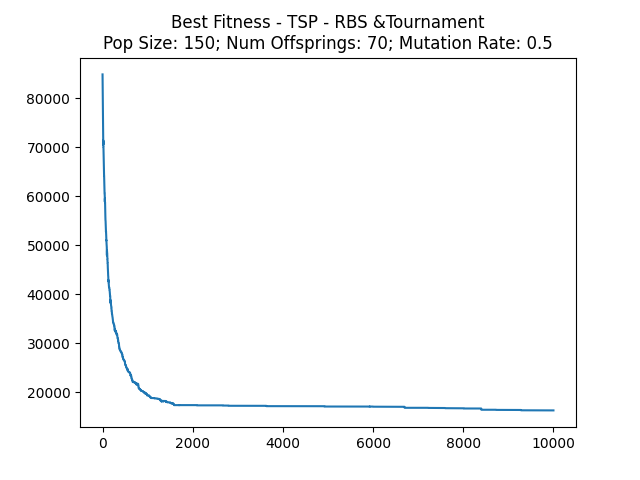
\includegraphics[scale=0.5]{../Analysis/BSF_TSP_1_2_150_70.png}
	      \includegraphics[scale=0.5]{../Analysis/ASF_TSP_1_2_150_70.png}
	      \\Initial fitness:  83413.0
	      \\Final fitness:  17525.0
	      \\Best Average Fitness: 15166.3
	      \\The value seems to converge, then have a steady value after 2000 generation.
	\item Case 6:\\
	      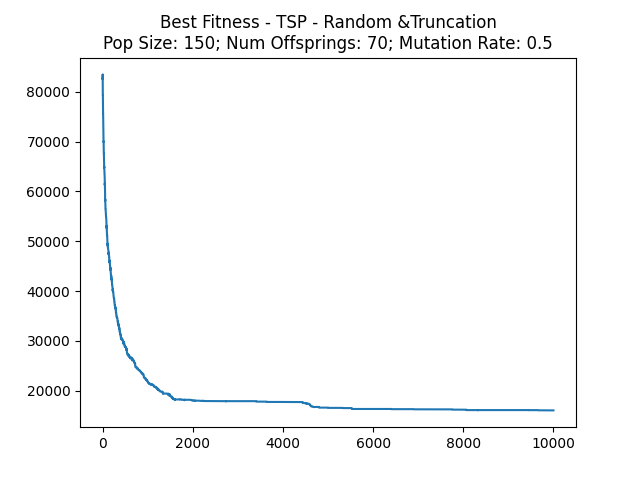
\includegraphics[scale=0.5]{../Analysis/BSF_TSP_4_3_150_70.png}
	      \includegraphics[scale=0.5]{../Analysis/ASF_TSP_4_3_150_70.png}
	      \\Initial fitness:  84648.0
	      \\Final fitness:  15208.0
	      \\Best Average Fitness: 16715.2
	      \\The value seems to converge, then have a steady value a bit after 2000 generation.
	\item Case 7:\\
	      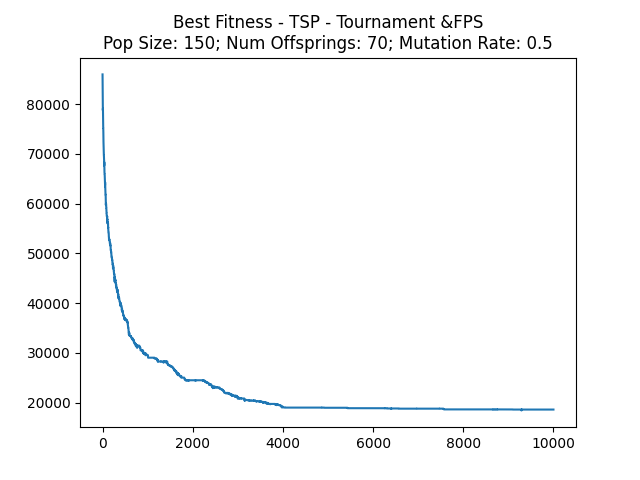
\includegraphics[scale=0.5]{../Analysis/BSF_TSP_2_0_150_70.png}
	      \includegraphics[scale=0.5]{../Analysis/ASF_TSP_2_0_150_70.png}
	      \\Initial fitness:  83917.0
	      \\Final fitness:  20122.0
	      \\Best Average Fitness: 18048.6
	      \\The value seems to converge, then have a steady value after 2000 generation.
	\item Case 8:\\
	      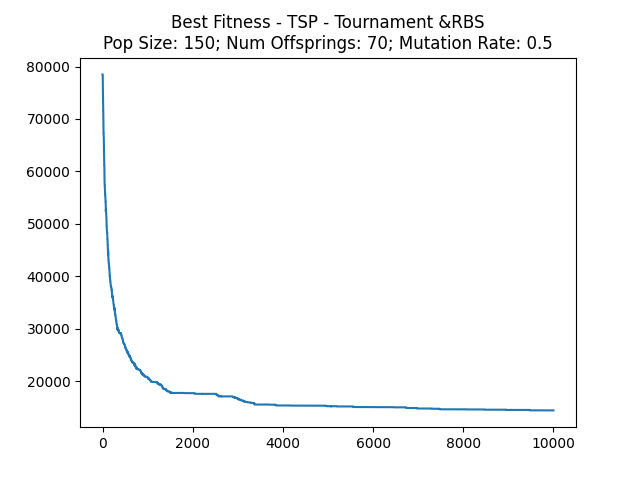
\includegraphics[scale=0.5]{../Analysis/BSF_TSP_2_1_150_70.png}
	      \includegraphics[scale=0.5]{../Analysis/ASF_TSP_2_1_150_70.png}
	      \\Initial fitness:  83759.0
	      \\Final fitness:  13788.0
	      \\Best Average Fitness: 15364.1
	      \\The value seems to converge, then have a steady value a bit after 4000 generation.
	\item Case 9:\\
	      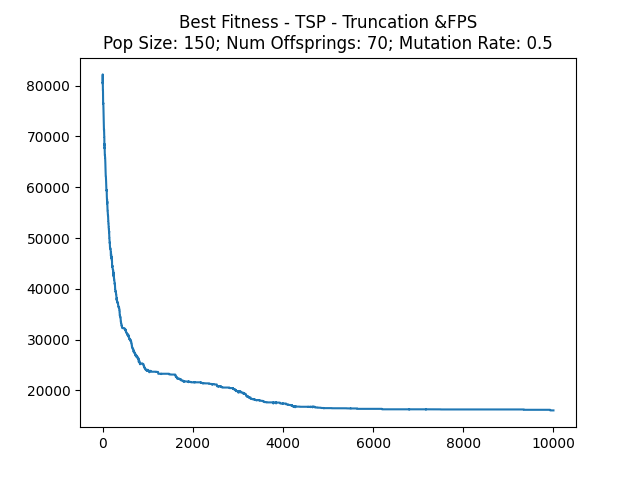
\includegraphics[scale=0.5]{../Analysis/BSF_TSP_3_0_150_70.png}
	      \includegraphics[scale=0.5]{../Analysis/ASF_TSP_3_0_150_70.png}
	      \\Initial fitness:  82137.0
	      \\Final fitness:  16927.0
	      \\Best Average Fitness: 15364.1
	      \\The value seems to converge, then have a steady value after 4000 generation.
\end{itemize}

\subsection*{Conclusion:}
We have the best output ins terms of BSF at case 8, where we used Binary Tournament and RBS, with the final fitness of 13788.0
\\And for the best output in terms of ASF we have a tie at case 8, where we used Truncation and Truncation,  with the final fitness of best average fitness of 15364.1 and case 9, where we used Truncation and FPS,  with the final fitness of best average fitness of 15364.1

\newpage


\section{Knapsack Problem}

\subsection{Best and Average Fitness So Far}

\begin{itemize}

	\item Case 0:\\
	      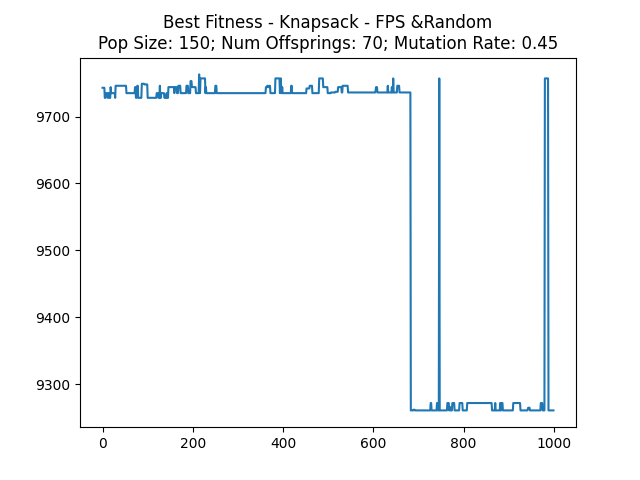
\includegraphics[scale=0.5]{../Analysis/BSF_Knapsack_0_4_150_70.png}
	      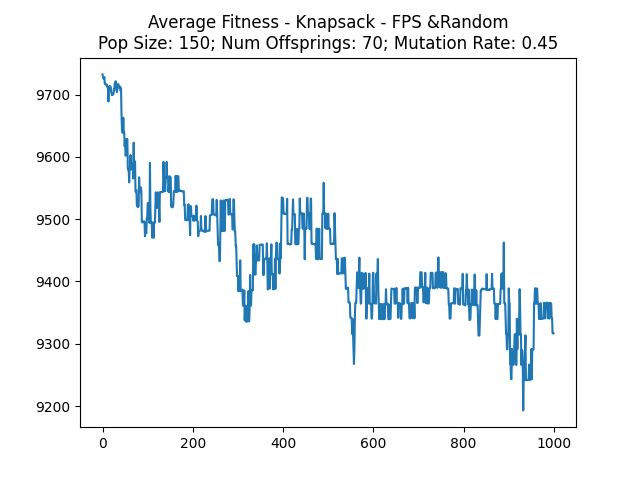
\includegraphics[scale=0.5]{../Analysis/ASF_Knapsack_0_4_150_70.png}
	      \\Initial fitness:  861
	      \\Final fitness:  826
	      \\Best Average Fitness: 876.1
	      \\We see that there are many random spikes, the plot doesnt seem to converge at any one value.
	      \\
	\item Case 1:\\
	      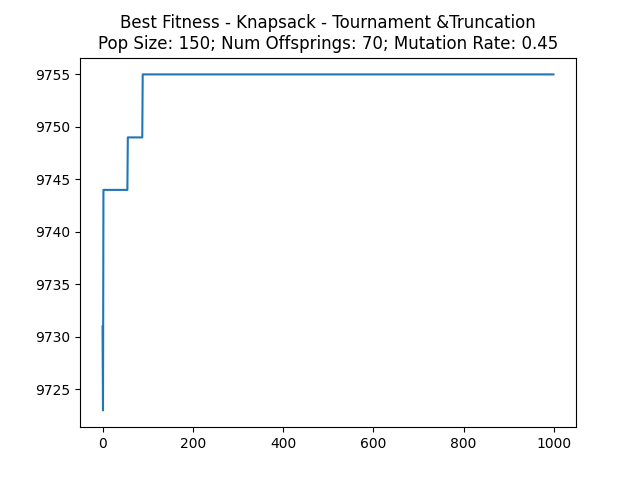
\includegraphics[scale=0.5]{../Analysis/BSF_Knapsack_2_3_150_70.png}
	      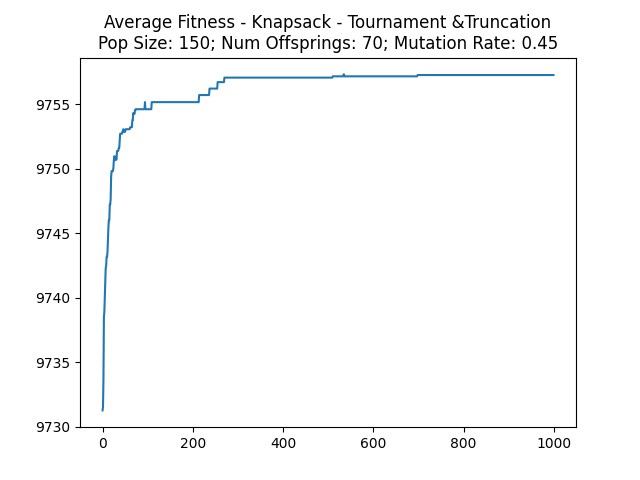
\includegraphics[scale=0.5]{../Analysis/ASF_Knapsack_2_3_150_70.png}
	      \\Initial fitness:  953
	      \\Final fitness:  1009
	      \\Best Average Fitness: 958.5
	      \\The values rapidly increases sometime before the 100th generation, then stays steady till sometime before the 600th generation, rapid increase and again get to a steady value till about 800 generation, then again a rapid increase and then stays steady and converges to out final value.
	\item Case 2:\\
	      \includegraphics[scale=0.5]{../Analysis/BSF_Knapsack_3_3_100_70.png}
	      \includegraphics[scale=0.5]{../Analysis/ASF_Knapsack_3_3_100_70.png}
	      \\Initial fitness:  843
	      \\Final fitness:  1009
	      \\Best Average Fitness: 959.15
	      \\The value rapidly increases till sometime around the 100th generation, then stays steady and converges at out final value.
	\item Case 3:\\
	      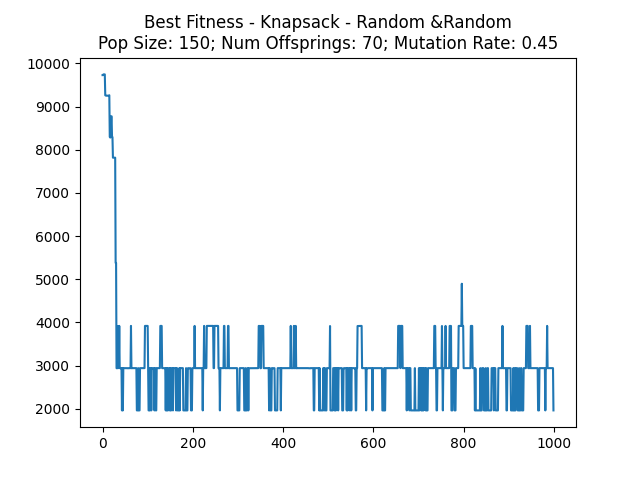
\includegraphics[scale=0.5]{../Analysis/BSF_Knapsack_4_4_150_70.png}
	      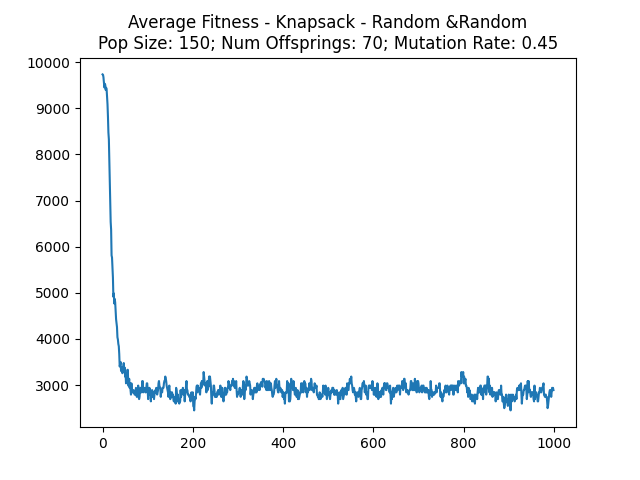
\includegraphics[scale=0.5]{../Analysis/ASF_Knapsack_4_4_150_70.png}
	      \\Initial fitness:  799
	      \\Final fitness:  136
	      \\Best Average Fitness: 861.75
	      \\The value falls down from our starting value, and then the plot seems to have random ups and down, and doesnt seem to converge at any perticular value
	\item Case 4:\\
	      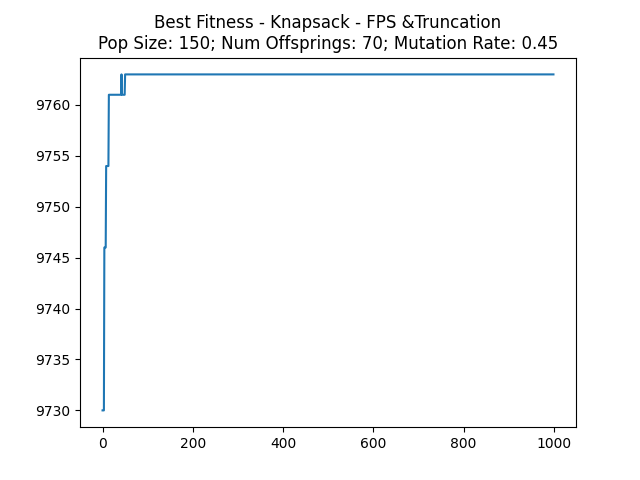
\includegraphics[scale=0.5]{../Analysis/BSF_Knapsack_0_3_150_70.png}
	      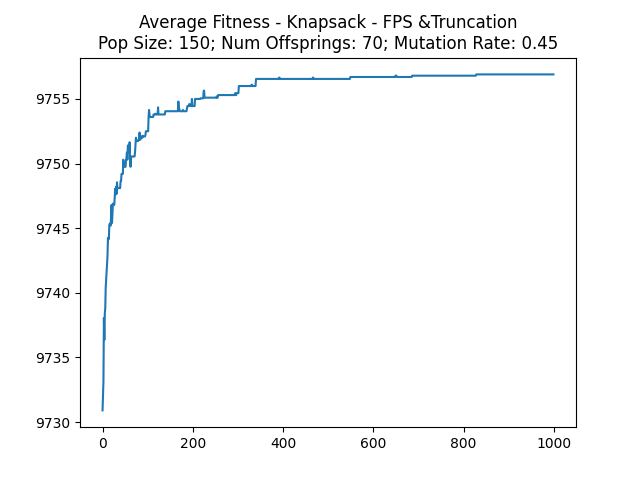
\includegraphics[scale=0.5]{../Analysis/ASF_Knapsack_0_3_150_70.png}
	      \\Initial fitness:  907
	      \\Final fitness:  963
	      \\Best Average Fitness: 939.5
	      \\ There seem to be a sudden spike and sudden down fall some generation after the 200th generation, the value increases till the aroung the 300th generation, then becomes steady and converges to out final answer.
	\item Case 5:\\
	      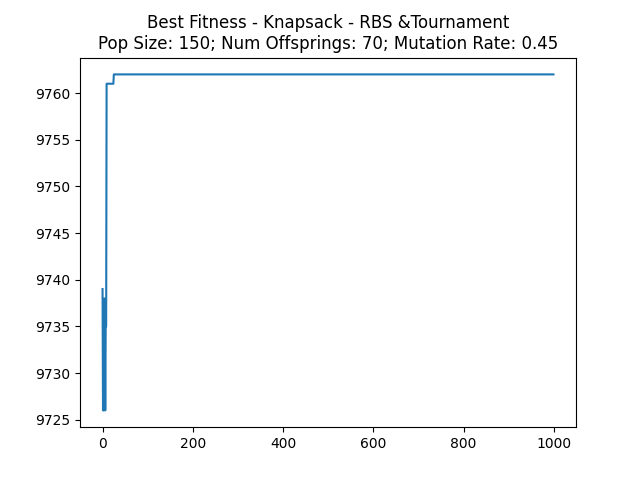
\includegraphics[scale=0.5]{../Analysis/BSF_Knapsack_1_2_150_70.png}
	      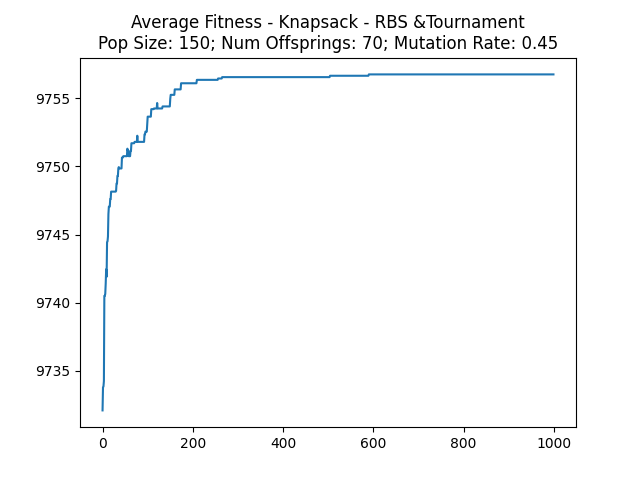
\includegraphics[scale=0.5]{../Analysis/ASF_Knapsack_1_2_150_70.png}
	      \\Initial fitness:  801
	      \\Final fitness:  826
	      \\Best Average Fitness: 956.85
	      \\The value rapidly increases in the first few generations then gets to a constant value.
	\item Case 6:\\
	      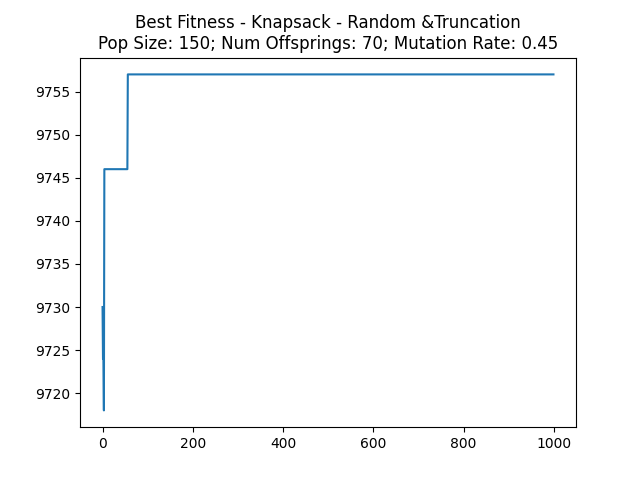
\includegraphics[scale=0.5]{../Analysis/BSF_Knapsack_4_3_150_70.png}
	      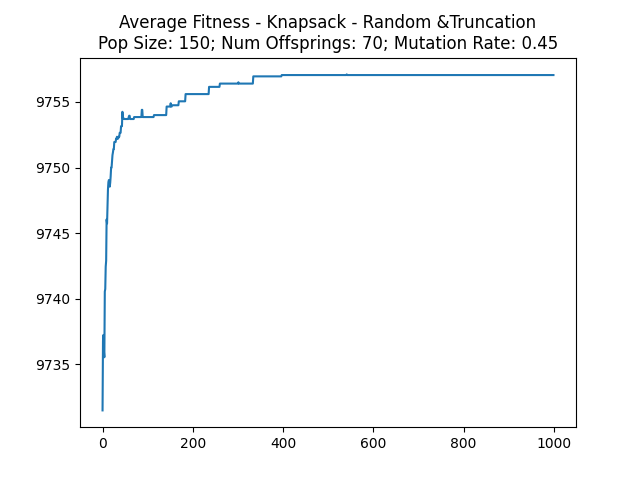
\includegraphics[scale=0.5]{../Analysis/ASF_Knapsack_4_3_150_70.png}
	      \\Initial fitness:  821
	      \\Final fitness:  913
	      \\Best Average Fitness: 932.8
	      \\ The value increase till about around the 100th generation, then becomes a steady value, and converges to out answer.
	\item Case 7:\\
	      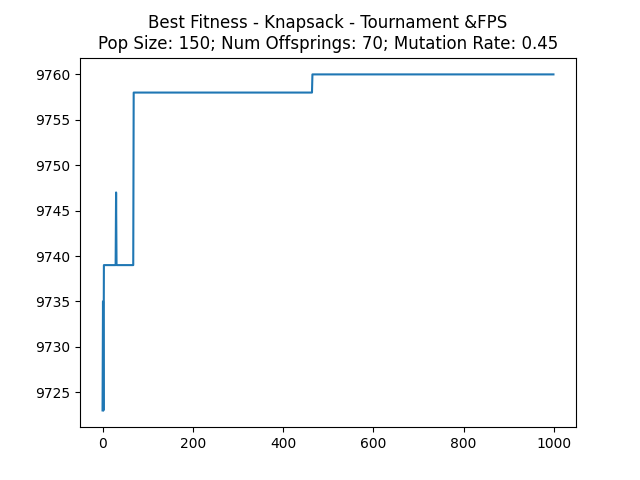
\includegraphics[scale=0.5]{../Analysis/BSF_Knapsack_2_0_150_70.png}
	      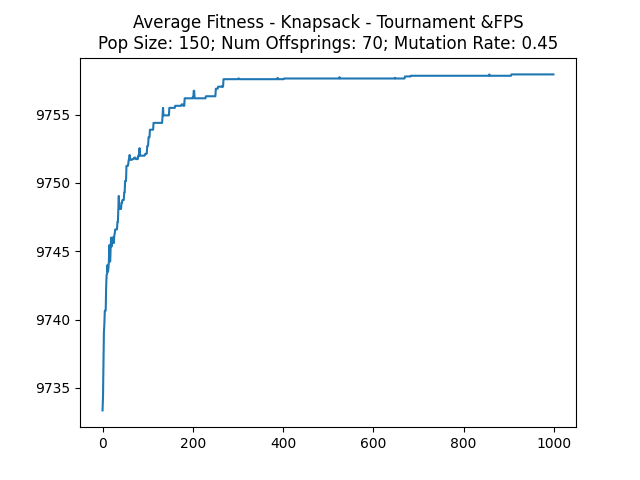
\includegraphics[scale=0.5]{../Analysis/ASF_Knapsack_2_0_150_70.png}
	      \\Initial fitness:  808
	      \\Final fitness:  826
	      \\Best Average Fitness: 951.7
	      \\The values behaves a bit randomly till about the 400th generation with some random spikes, after which it seems to converge to our final value.
	\item Case 8:\\
	      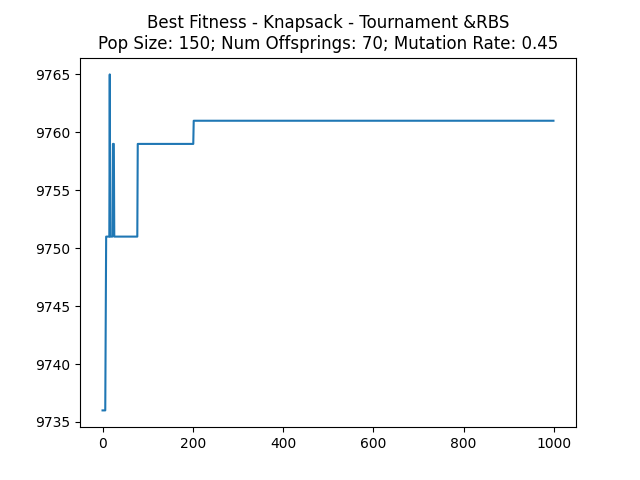
\includegraphics[scale=0.5]{../Analysis/BSF_Knapsack_2_1_150_70.png}
	      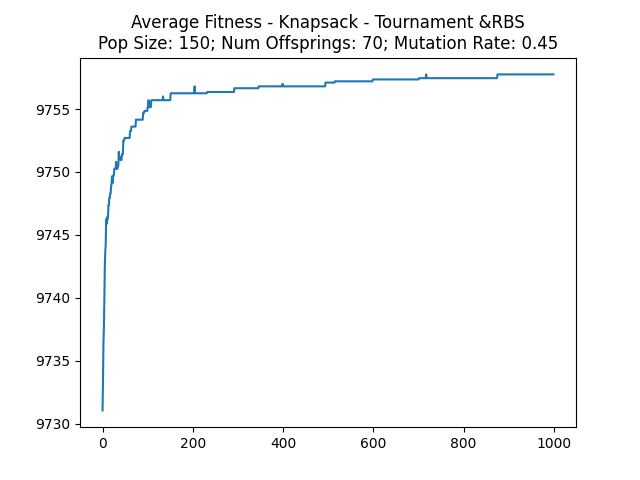
\includegraphics[scale=0.5]{../Analysis/ASF_Knapsack_2_1_150_70.png}
	      \\Initial fitness:  818
	      \\Final fitness:  1013
	      \\Best Average Fitness: 937.05
	      \\the values increases till sometime around the 100th generation, after which seems to converge become steady at our final value.
	\item Case 9:\\
	      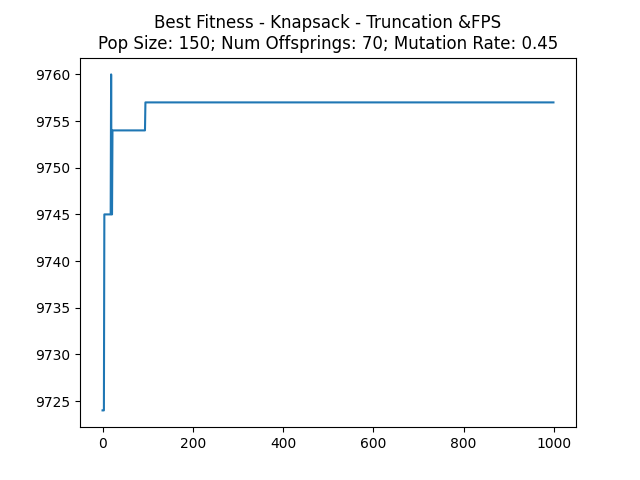
\includegraphics[scale=0.5]{../Analysis/BSF_Knapsack_3_0_150_70.png}
	      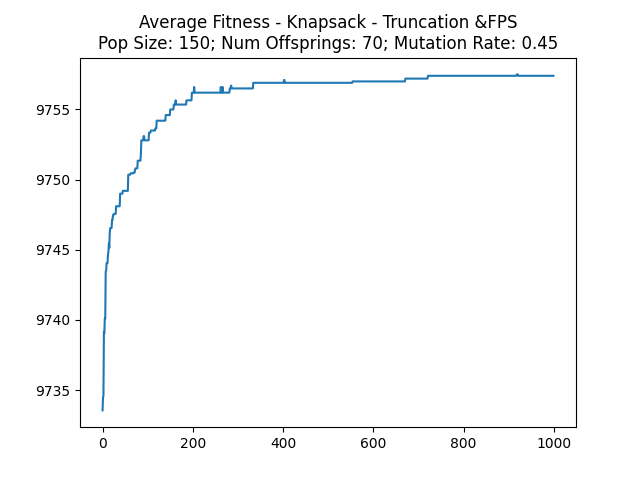
\includegraphics[scale=0.5]{../Analysis/ASF_Knapsack_3_0_150_70.png}
	      \\Initial fitness:  804
	      \\Final fitness:  839
	      \\Best Average Fitness: 952.55
	      \\the values increases till sometime around the 100th generation, with one raondom spike in between, after which seems to converge become steady at our final value.
\end{itemize}

\subsection*{Conclusion:}
We have the best output ins terms of BSF at case 8, where we used Binary Tournament and RBS, with the final fitness of 1013
\\And the best output in terms of ASF at case 2, where we used Truncation and Truncation,  with the final fitness of best average fitness of 959.15

\newpage





\section{Graph Coloring Problem}

\subsection{Best and Average Fitness So Far}


\begin{itemize}

	\item Case 0:\\
	      \includegraphics[scale=0.5]{../Analysis/BSF_Graph_Coloring_0_4_130_70.png}
	      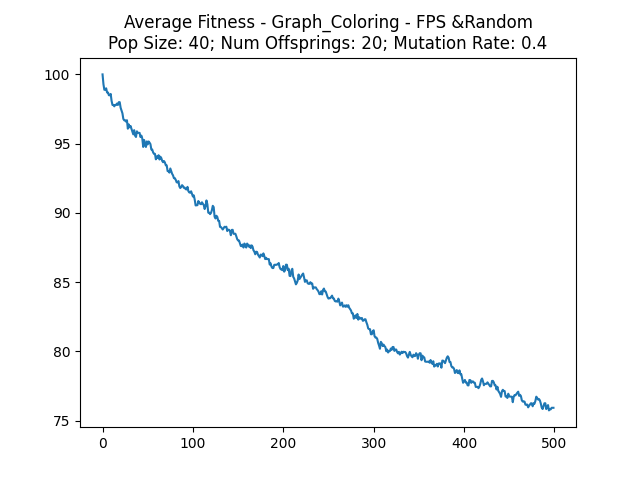
\includegraphics[scale=0.5]{../Analysis/ASF_Graph_Coloring_0_4_40_20.png}
	      \\Initial fitness:  100.0
	      \\Final fitness:  60.0
	      \\Best Average Fitness: 73.02925334197116
	      \\We see that there are many random spikes, the plot doesnt seem to converge at any one value. Although in the begining the general trend seems to be decreasing, but after 750 generations it seems to be purely random.
	      \\
	\item Case 1:\\
	      \includegraphics[scale=0.5]{../Analysis/BSF_Graph_Coloring_2_3_150_70.png}
	      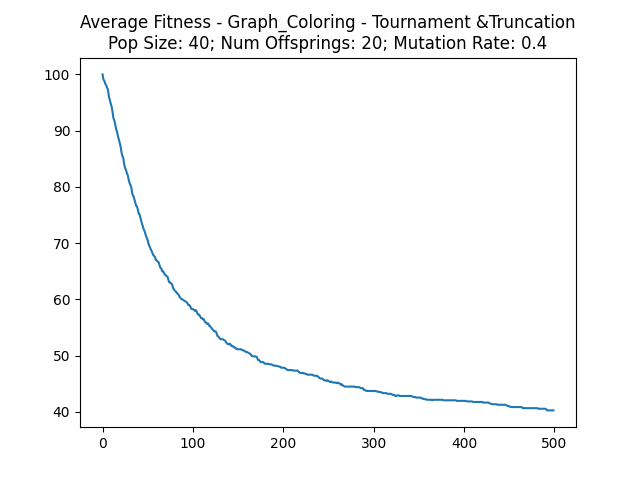
\includegraphics[scale=0.5]{../Analysis/ASF_Graph_Coloring_2_3_40_20.png}
	      \\Initial fitness:  100.0
	      \\Final fitness:  31.0
	      \\Best Average Fitness: 40.363824263903076
	      \\The values rapidly decreases till about the 250th generation, after which it slowly converges to our value, and seem to get constant after around the 1500th generation.
	\item Case 2:\\
	      \includegraphics[scale=0.5]{../Analysis/BSF_Graph_Coloring_3_3_120_70.png}
	      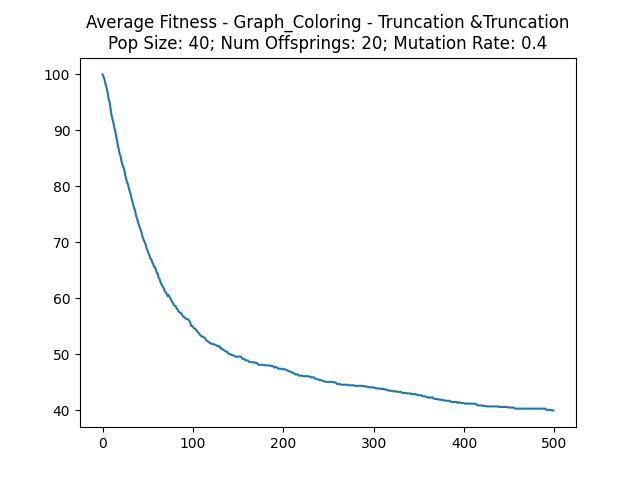
\includegraphics[scale=0.5]{../Analysis/ASF_Graph_Coloring_3_3_40_20.png}
	      \\Initial fitness:  100.0
	      \\Final fitness:  31.0
	      \\Best Average Fitness: 39.22761681380331
	      \\The values rapidly decreases till about the 250th generation, after which it slowly converges to our value, and seem to get constant after around the 1500th generation.
	\item Case 3:\\
	      \includegraphics[scale=0.5]{../Analysis/BSF_Graph_Coloring_4_4_150_70.png}
	      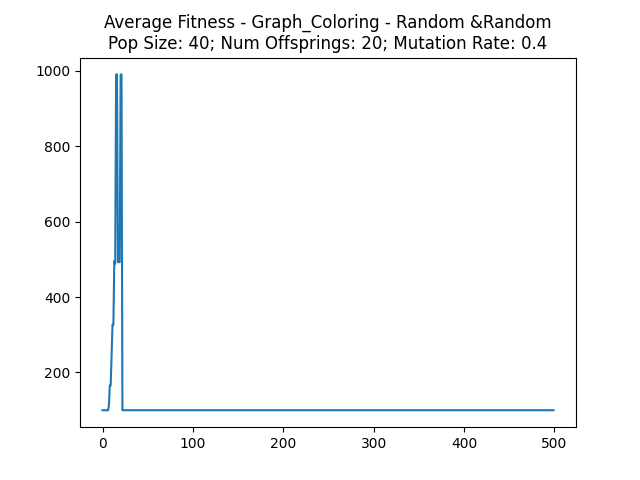
\includegraphics[scale=0.5]{../Analysis/ASF_Graph_Coloring_4_4_40_20.png}
	      \\Initial fitness:  100.0
	      \\Final fitness:  100
	      \\The values seem to be constant at about 100
	\item Case 4:\\
	      \includegraphics[scale=0.5]{../Analysis/BSF_Graph_Coloring_0_3_150_70.png}
	      \includegraphics[scale=0.5]{../Analysis/ASF_Graph_Coloring_0_3_40_20.png}
	      \\Initial fitness:  100.0
	      \\Final fitness:  30.0
	      \\Best Average Fitness: 41.93187519382236
	      \\The values rapidly decreases till about the 250th generation, and seem to get constant after around the 1000th generation, seems to have another fall just before our 2000th genration and ger to out final value.
	\item Case 5:\\
	      \includegraphics[scale=0.5]{../Analysis/BSF_Graph_Coloring_1_2_150_70.png}
	      \includegraphics[scale=0.5]{../Analysis/ASF_Graph_Coloring_1_2_40_20.png}
	      \\Initial fitness:  100.0
	      \\Final fitness:  35.0
	      \\Best Average Fitness: 40.31416937470411
	      \\The values rapidly decreases till about a bit before the 250th generation, after which it slowly converges to our value, and seem to get constant after around the 1250th generation.
	\item Case 6:\\
	      \includegraphics[scale=0.5]{../Analysis/BSF_Graph_Coloring_4_3_150_70.png}
	      \includegraphics[scale=0.5]{../Analysis/ASF_Graph_Coloring_4_3_40_20.png}
	      \\Initial fitness:  100.0
	      \\Final fitness:  30.0
	      \\Best Average Fitness: 41.346202280602
	      \\The values rapidly decreases till about a bit before the 250th generation, after which it slowly converges to our value.
	\item Case 7:\\
	      \includegraphics[scale=0.5]{../Analysis/BSF_Graph_Coloring_2_0_150_70.png}
	      \includegraphics[scale=0.5]{../Analysis/ASF_Graph_Coloring_2_0_40_20.png}
	      \\Initial fitness:  100.0
	      \\Final fitness:  36.0
	      \\Best Average Fitness: 43.998039470317764
	      \\The values rapidly decreases till about a bit before the 250th generation, after which it slowly converges to our value, and seem to get constant after around the 1500th generation.
	\item Case 8:\\
	      \includegraphics[scale=0.5]{../Analysis/BSF_Graph_Coloring_2_1_150_70.png}
	      \includegraphics[scale=0.5]{../Analysis/ASF_Graph_Coloring_2_1_40_20.png}
	      \\Initial fitness:  100.0
	      \\Final fitness:  33.0
	      \\Best Average Fitness: 40.4358386574539
	      \\The values rapidly decreases till about the 250th generation, and seem to get constant after around the 1250th generation, seems to have another fall after 1750th generation and get to out final value.
	\item Case 9:\\
	      \includegraphics[scale=0.5]{../Analysis/BSF_Graph_Coloring_3_0_150_70.png}
	      \includegraphics[scale=0.5]{../Analysis/ASF_Graph_Coloring_3_0_40_20.png}
	      \\Initial fitness:  100.0
	      \\Final fitness:  32.0
	      \\Best Average Fitness: 43.4672614706304
	      \\The values rapidly decreases till about a bit before the 250th generation, after which it slowly converges to our value.
\end{itemize}


\subsection*{Conclusion:}
For the best output in terms of BSF we have a tie at case 4, where we used FPS and Truncation, and case 6, where we used, with the final fitness of 30

\\And the best output in terms of ASF at case 1, where we used FPS and Random , with the final fitness of best average fitness of 40.363824263903076


\end{document}